\subsubsection{Top \dword{fc} penetration}
\label{sec:lasertopfcpen}

Given that the \dword{fc} profiles are \SI{4.6}{\cm} wide with only a small \SI{1.4}{\cm} gap between them, the shadows 
%caused 
produced when the laser source is outside the \dword{fc} are substantial. We estimate that the maximum angle at which beams can go through is about \ang{45}. Given the limitations of the region above the \dword{fc}, especially the geometry of the ground plane, it is likely that the mirror cannot be placed much higher up than \SI{40}{\cm} away from the \dword{fc}. This means that, close to the top \dword{fc}, the covered region will be only about \SIrange{40}{60}{\cm} long, in each \SI{3.6}{\m} long drift volume. 
%Considering 
For simplicity considering no limitations to movement along the direction of the \dword{fc} profiles, 
%that means that 
only about \num{10} to \SI{15}{\%} of the top area of the \dword{fc} would be covered by the laser system. On the bottom \dword{fc}, that ratio would be slightly higher, corresponding to the ratio of gap (\SI{1.4}{\cm}) to total (\SI{6}{\cm}) width, i.e. about \SI{23}{\%}.

Penetration of the \dword{fc} would eliminate those shadows and allow for a practically unimpeded coverage. Fig.~\ref{fig:laser_fcpenetration} shows a possible way to accomplish this for the top-of-TPC ports~\cite{bib:yu2019a}. A CAD model of the \dword{sbnd} laser calibration system periscope was used as 
%an example the design 
reference design for \dword{dune}. The \dword{sbnd} periscope, when rotating over its axis, requires a \SI{12}{\cm} diameter circular region free of impediments. In order to take into account a tolerance for the estimated \SI{0.3}{\%} shrinkage of the \dword{fc} at cryogenic temperatures, we chose an opening of \num{3} profiles, equivalent to \SI{18}{\cm}.

\begin{dunefigure}[Laser periscope penetrating the field cage]{fig:laser_fcpenetration}
{CAD drawing of one way the periscope could penetrate the \dword{fc}~\cite{bib:yu2019a}.}
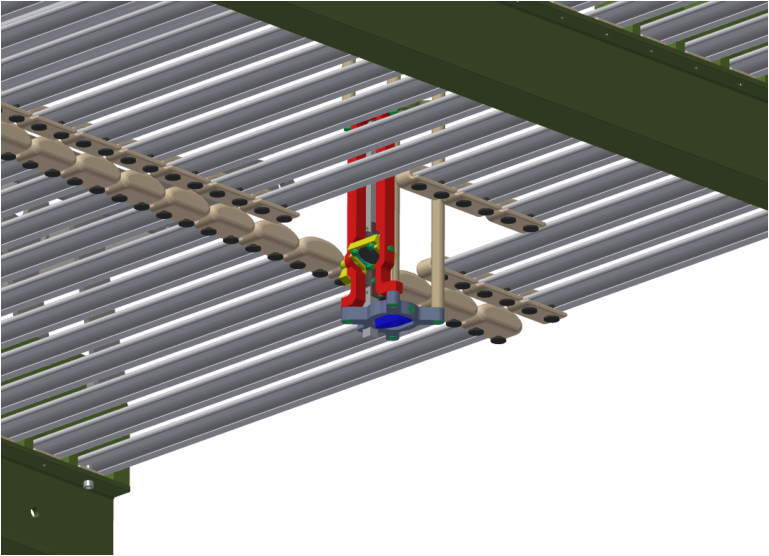
\includegraphics[width=0.8\linewidth]{laser_fcpenetration.pdf}
\end{dunefigure}

Simulations of the effect of \dword{fc} penetrations on the \efield were carried out~\cite{bib:yu2017b}, and are illustrated in Figure~\ref{fig:efield_penetration_boyu2017}. These have shown that the effect of a \num{12}$\times$\SI{12}{\square\cm} (equivalent to \num{2} profiles) opening, located at \SI{40}{\cm} (along the $x$ direction) from the \dword{apa}, is small and tolerable, since the unusable volume would be about \SI{2.2}{\litre}. These simulations need to be redone with a larger opening of \num{18}$\times$\SI{18}{\square\cm} (\num{3} profiles).

\begin{dunefigure}[Simulation of impact on \efield of \dword{fc} penetration]{fig:efield_penetration_boyu2017}
{Simulation of the effect on the \efield of a laser periscope penetration of the \dword{fc}. In this case, an opening of only two profiles was considered.}
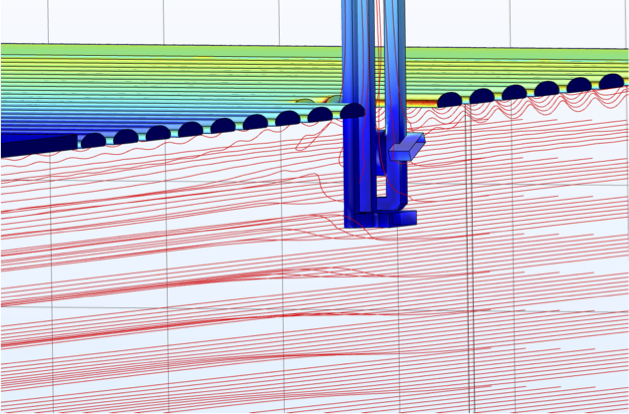
\includegraphics[width=0.8\linewidth]{efield_penetration_boyu2017.png}
\end{dunefigure}




%%%%%%%%%%%%%%%%%%%%%%%%%%%%%%%%%%%%%%%%%%%%%%%%%%%%%%%%%%%%%%%%

\subsubsection{End-wall coverage enhancement}

The eight calibration ports closer to the end-walls (four on each side) are not positioned on top of the \dword{tpc}, but located about \SI{40}{\cm} away from the \dword{fc} along the $z$ direction.
Therefore the same solution proposed in the previous section is not directly applicable.

The disadvantages of the baseline system in terms of volume coverage have been described above, and apply to the end-wall ports as well. Two different ideas on how to improve the laser beam coverage from these eight ports are being considered and are described in the following paragraphs.

%\paragraph{Horizontal track along end-wall}

%The baseline design is based on laser entry points in which the movement of the steering mirror has two angular degrees of freedom.
%A possible alternative design would change that end part of the system so that there is a translation and a rotation movement. At the end of the vertical periscope, a mirror at a \ang{45} angle would send the beam horizontally, perpendicular to the \dword{apa}/\dword{cpa}, and externally to the field cage. A horizontal track, installed in that same direction, would allow the translation movement of a secondary mirror (or two of them, one on each side), mounted with an angle of \ang{45} with respect to the incident beam. This allows the mirror to be aligned with the \SI{1.4}{\cm} wide gaps between the \dword{fc} profiles. This second mirror would have a rotation movement, around the same axis, keeping the \ang{45} angle to the beam, but causing its reflection to sweep a vertical plane. Figure~\ref{fig:Laser_alternative2} provides an illustration of the mirror movements in this arrangement.

%\begin{dunefigure}[Sketch of horizontal track for alternative laser beam movement ]{fig:Laser_alternative2}
%{Sketch of the beam array using end-wall horizontal track arrangement. The two planes on either side of the laser tracks (magenta) are cathode and anode.}
%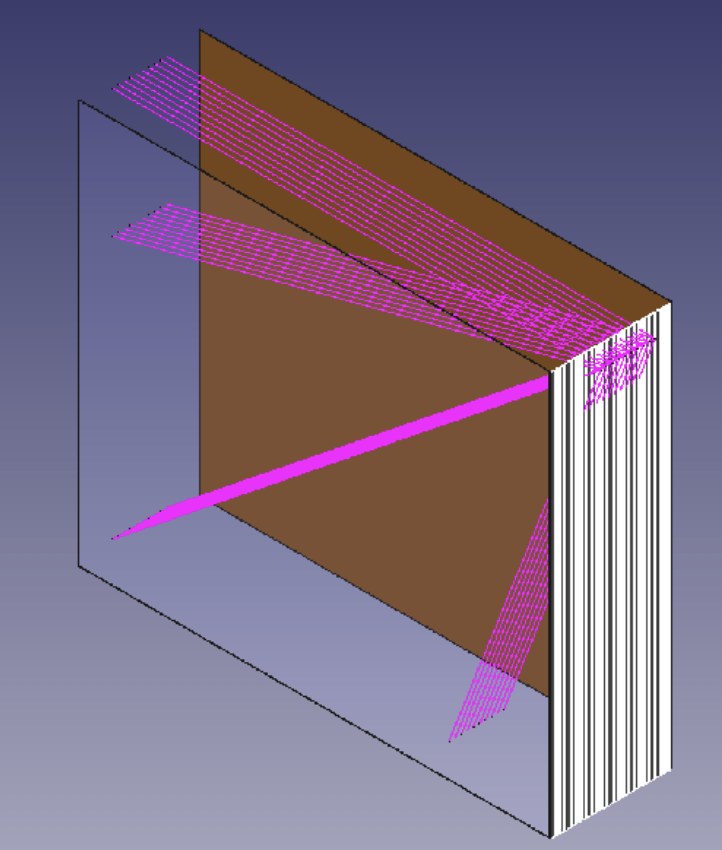
\includegraphics[width=0.5\linewidth]{Laser_alternative2.png}
%\end{dunefigure}

%In terms of cryostat penetration, the design of the feedthrough and periscope would follow the baseline. The horizontal track could hang down from the calibration ports, and long plastic threaded rods supported by it could be used to transmit translation and rotation movement to the secondary mirror. It appears quite challenging to implement such a system for this translation and rotation movement, that meets the \efield and cryogenic constraints within the \dword{dune} cryostat, as well as the mechanical precision requirements.
%Still, if possible, this solution would have very good TPC coverage (even if somewhat limited by the horizontal \dword{fc} support bars), and possibly allow for only one laser to be used at each end-wall.

{\it End-wall \dword{fc} penetration:}\\ 
The best possible \dword{tpc} coverage should be achieved with \dword{fc} penetration. A conceptual plan for this, sketched in Figure~\ref{fig:laser-alt-ewpen1} would be to build L-shaped periscopes that, using Cardan joints, would change the periscope rotation axis (and the translation stage movement) from vertical to horizontal, in order to actuate the mirror inside the \dword{tpc}. In addition to solving the mechanical issues associated with the L-shaped transmission, the effect of such openings on the \efield still needs to be carefully studied, since the end-wall calibration ports are not located close to the \dwords{apa}, but are at about \SI{2}{\m} in the drift direction, so their impact is higher than in the case described in Section~\ref{sec:lasertopfcpen}.

\begin{dunefigure}[Sketch of L-shaped laser periscope for end-wall \dword{fc} penetration]{fig:laser-alt-ewpen1}
{Sketch of the laser beam L-shaped periscope arrangement for horizontal end-wall \dword{fc} penetration.}
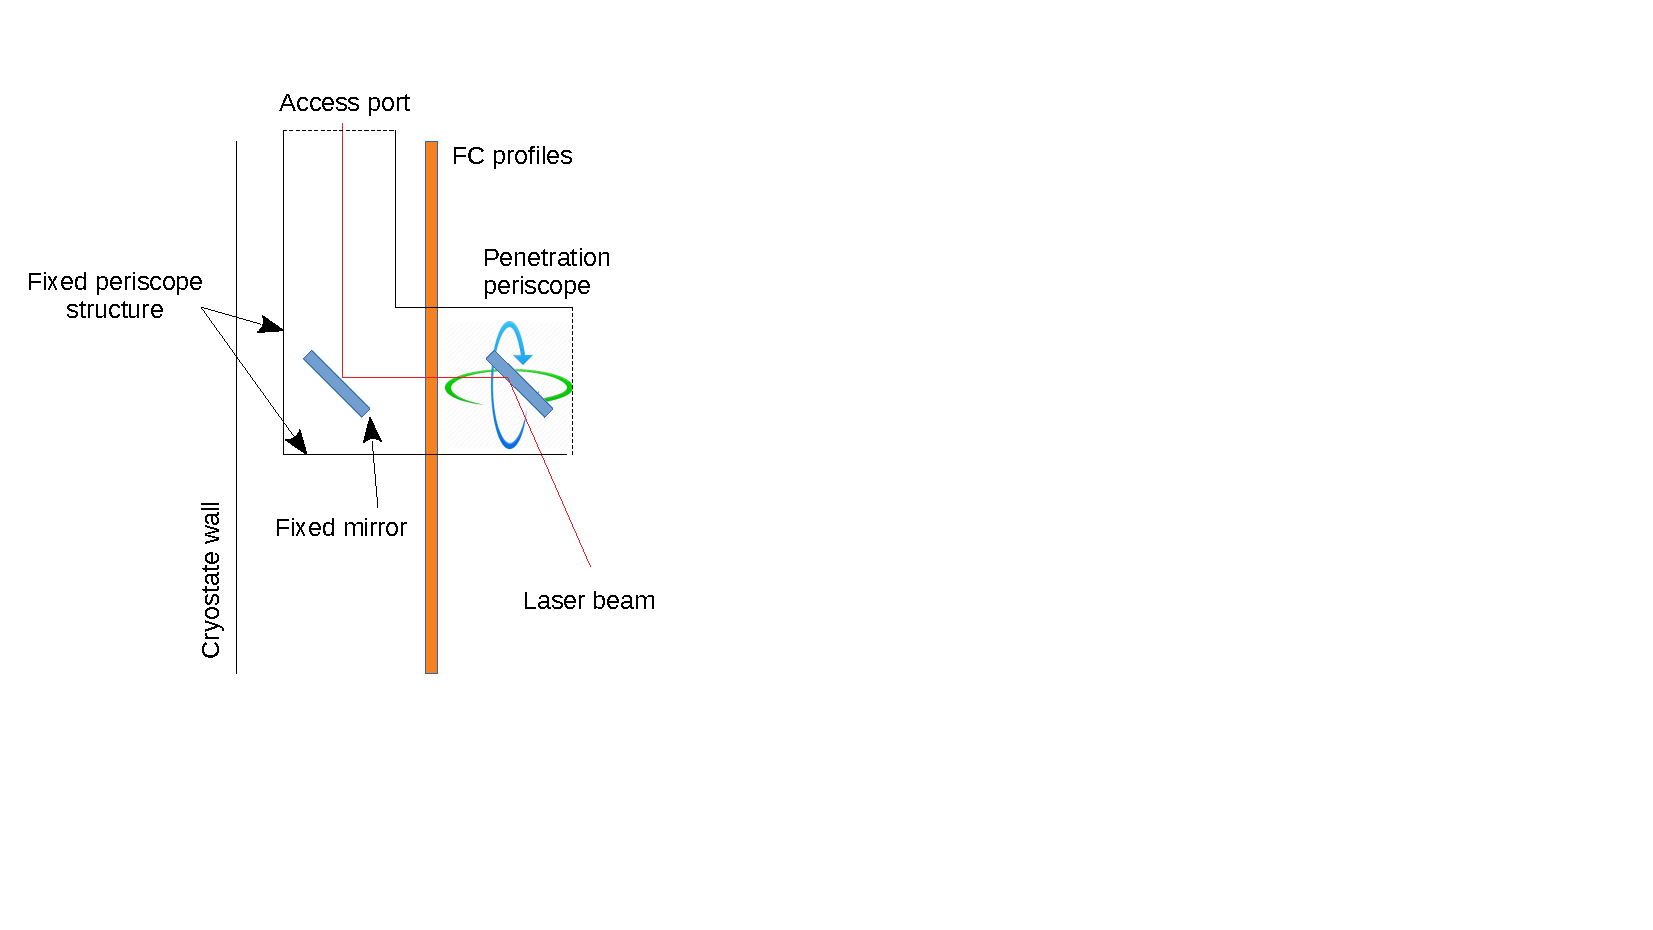
\includegraphics[width=0.5\linewidth]{laser-alt-ewpen1.pdf}
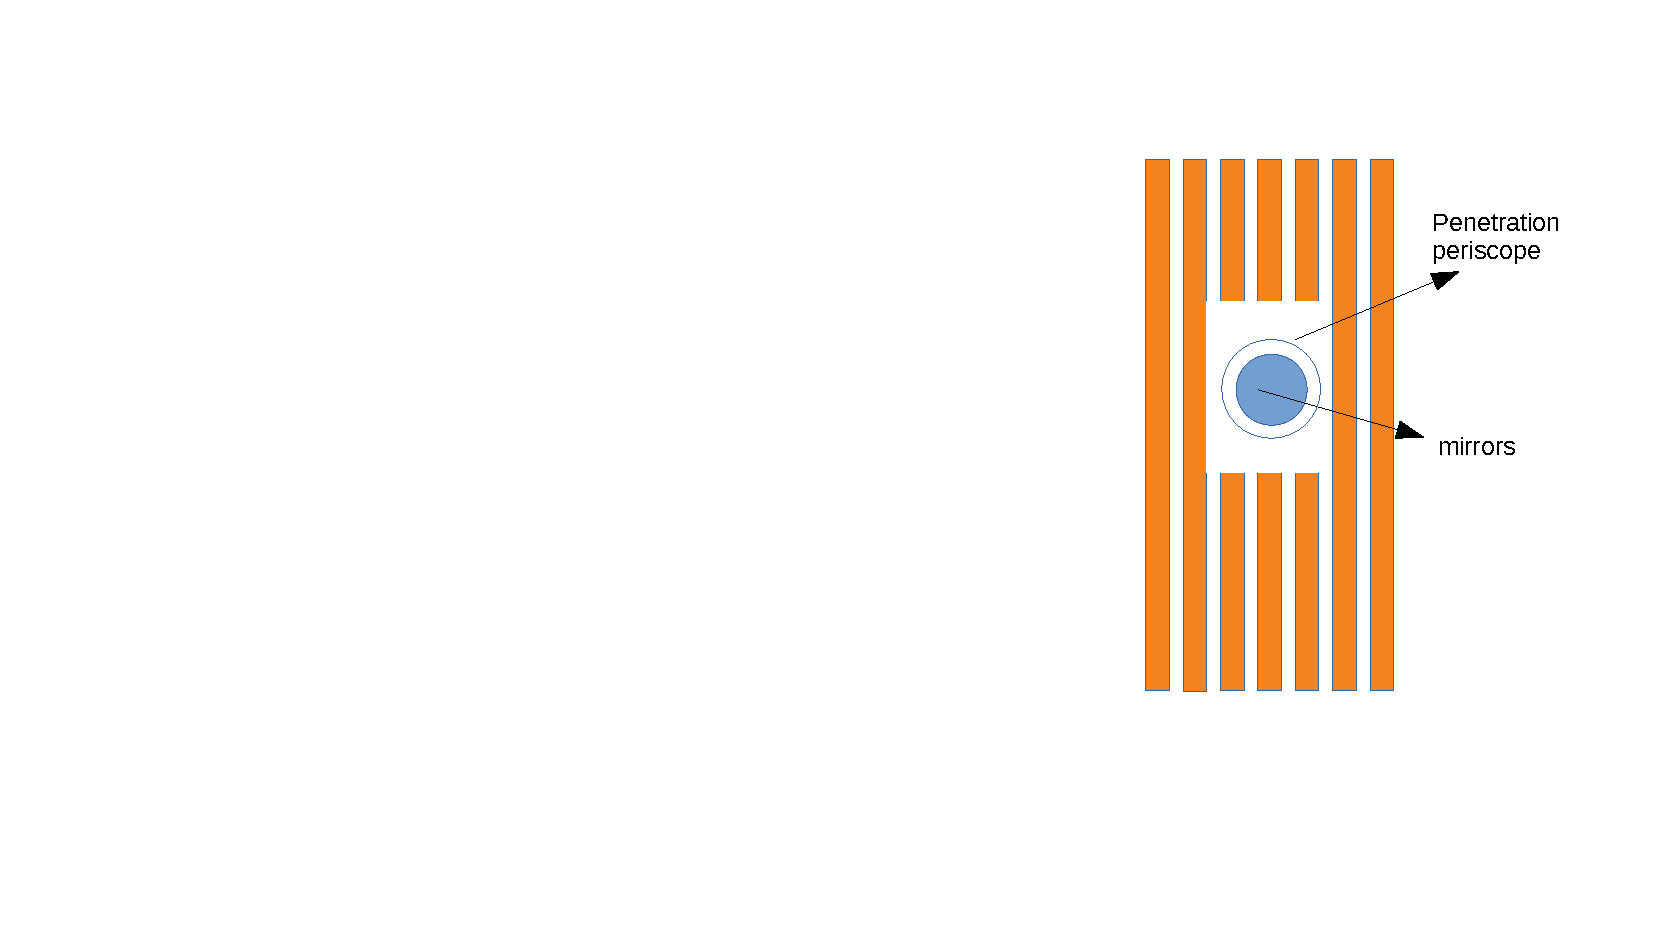
\includegraphics[width=0.3\linewidth]{laser-alt-ewpen2.pdf}
\end{dunefigure}

{\it Additional rotation stage:}\\ 
A second alternative design for the end-wall ports does not require \dword{fc} penetration
%or long horizontal tracks. 
The periscope is exactly the same as the baseline design but, at the top of the calibration port, is mounted on a flange that has an additional rotation degree of freedom. Figure~\ref{fig:laser_extrarotation} presents a rough sketch of the concept. The \SI{250}{\milli\m} diameter calibration port has on top of it the main rotary flange that, itself, has another \SI{150}{\milli\m} port off-centered by \SI{40}{\milli\m} with respect to the main port. On this smaller port, a secondary rotary flange is installed and it is this one that holds the laser periscope, including the optical feedthrough and the linear stage for mirror movement. When the main flange rotates, the periscope also moves along a circular (\SI{40}{\milli\m} diameter) trajectory. Consequently, within the cryostat, the relative position between the beam mirror and the \dword{fc} profiles changes as well, and so the shadowed regions also change. Using different main rotary flange angles, it should be possible to locate the mirror in enough different positions in order to cover all the previously shadowed angles.

\begin{dunefigure}[Sketch of the rotary flange arrangements on the end-wall calibration ports]{fig:laser_extrarotation}
{Sketch of the rotary flange arrangements on the end-wall calibration ports.}
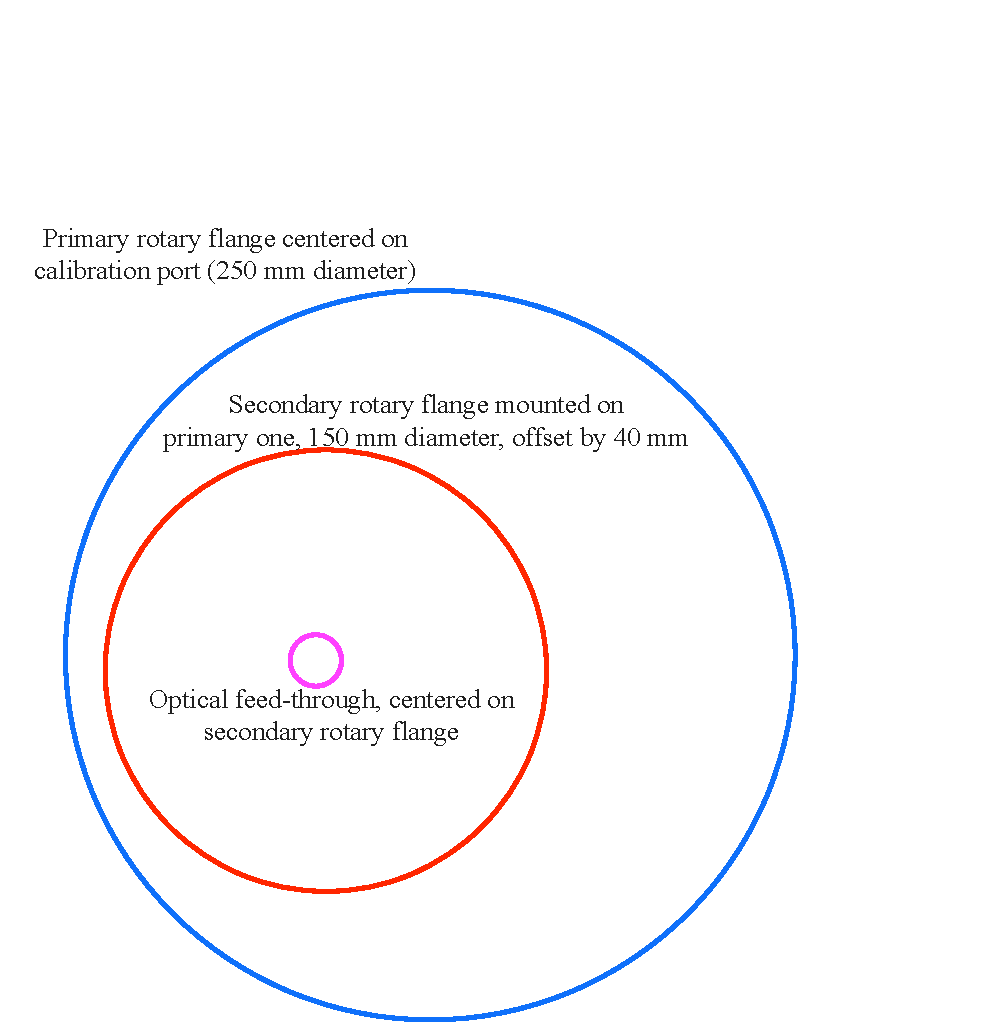
\includegraphics[width=0.6\linewidth]{laser_extrarotation.pdf}
\end{dunefigure}


%In terms of cryostat penetration, the design of the feedthrough and periscope would follow the baseline one, but the $\theta$ angle would be practically always \ang{45}, with only minor adjustments, and the phi angle would flip between \ang{0} and \ang{180}. 
%ref Newport mirror for 266 nm, https://www.newport.com/p/10QM20HM.75
%%The reflected beam is parallel to the \dword{fc} wall and perpendicular to the \dword{apa}. There would have to be a new \num{14}~m long tray for the movement of the secondary mirror(s). 
%Long plastic threaded rods could be used for the movement along the tray. Rotation of the first rod would push/pull a small platform along the tray, and the rotation of the second rod is transmitted to a mechanism on that platform to achieve the rotation around the $x$ axis.

%The \dword{fc} profiles are \SI{4.6}{\cm} wide with a \SI{1.4}{\cm} gap between them. That's the gap close to which the mirror needs to stop. That means that there is a finite amount of $x$ values where we can position the mirror, effectively every \SI{6}{\cm}. In order to correct for possible \dword{fc} shifts, one can use the laser positioning system to see if beam is passing to the other side. Choosing the $z$ coordinate of the tray to be located close to an edge of the drift volume, the angular range of movement needed to fully cover a vertical plane with the rotation of the mirror is only \ang{90}.

%This mirror movement system has the following advantages:
%\begin{itemize}
%\item good coverage of most of the \dword{tpc} active volume, even  from outside the \dword{fc};
%\item the same calibration port laser can illuminate all drift volumes;
%\item with the beam always parallel to the \dword{apa}, especially the \dword{pds}, less risk of hitting the \dword{pds}
%directly or by reflecting from the cathode although reflections from the \dword{fc} profiles are still possible).
% * <maneira@gmail.com> 2018-10-22T07:07:38.035Z:
% 
% is there any calculation of the space charge effect of the laser beams themselves? the number of tracks we want to use is pretty high.
% 
% ^.
%\end{itemize}

%The reference system does have the following possible disadvantages:
%\begin{itemize}
%\item Construction requires more moving parts and movement transmitted at long distances, so the mechanical precision may be more challenging to achieve the same precision as in the baseline;
%\item The \dword{fc} profiles may shift during cooling, creating a need to fine-tune the alignment of the mirror with the \dword{fc} gaps. This can be done with the laser positioning system described in Section~\ref{sec:calib-laser-pos};
%% JM %% include Jelena's text about it and reference it here.
 
%\end{itemize}
